\documentclass[a4paper, notitlepage]{report}
\title{Smartphone Audio Acquisition and Synchronization Using an Acoustic Beacon}
\author{\sffamily\small S. Bosma, R. Smeding}
\date{}
% All imports needed for file

% General
\usepackage[a4paper,top=1.25in,right=1in,bottom=1.25in,left=1in]{geometry}
\usepackage[utf8]{inputenc}
\usepackage[T1]{fontenc}
\usepackage{textcomp}
\usepackage[bitstream-charter]{mathdesign}
\usepackage{cite}

\usepackage{import}
\usepackage{standalone}
\usepackage{epstopdf}



% Math
\usepackage{amsmath}	% some standard math functions
%\usepackage{amssymb}	% more mathematical symbols
\usepackage{amsbsy}	% enable bold mathematics
\usepackage{bm}
%\usepackage{amsthm}	% enable theorem statements
\usepackage{trfsigns} 	% symbols for transforms

% Text formatting
\usepackage{fancyhdr}	% allow more control over page headers/footers
\usepackage{enumitem}	% allow control over enumerate, itemize, description
\usepackage{setspace}	% allow control over spacing
\usepackage{lastpage}	% provide label for last page in document
\usepackage{sectsty}	% allow control over section styling
\usepackage{url}

% Floats
\usepackage{xcolor}		% enable use of colors
\usepackage{graphicx}		% enable graphics
\usepackage{float}		% enable floats
\usepackage[section]{placeins}	% prevent floats from moving past e.g. sections
\usepackage[small, bf, hang, figurename=Fig.]{caption}	% enable captions for floats (images etc.)
\captionsetup{width=.8\textwidth} % captions not too wide
\usepackage{subcaption}		% enable subcaptions for floats (images etc.)
\usepackage[nottoc]{tocbibind}		% put more stuff in TOC

% Styling data
\pagestyle{fancyplain}

% Title page
\makeatletter
\let\inserttitle\@title
\makeatother

% Page header
\setlength{\headwidth}{\textwidth}
\lhead{} % leave left header empty
\chead{}
\rhead{} % leave right header empty
\lfoot{} % leave left footer empty
\cfoot{} % leave center footer empty
\rfoot{}
\renewcommand{\headrulewidth}{0.3pt}
\renewcommand{\footrulewidth}{0pt}

% Section, equation and figure numbering
\usepackage{chngcntr} 
\counterwithout{figure}{chapter}
\renewcommand{\thechapter}{\Roman{chapter}}
\renewcommand{\thesection}{\Roman{chapter}.\arabic{section}}
\renewcommand{\thesubsection}{\Roman{chapter}.\arabic{section}.\arabic{subsection}}
\renewcommand{\thesubsubsection}{\alph{subsubsection})}
\renewcommand{\thefigure}{\arabic{figure}}
\renewcommand{\thesubfigure}{\alph{subfigure}}
\renewcommand{\theequation}{\thechapter--\arabic{equation}}
\setcounter{tocdepth}{1}
\captionsetup[figure]{labelsep=period}

% Nice enumerations
\newlist{enum}{enumerate}{1}
\setlist[enum]{label=\textbf{[\arabic*]}} % \arabic or \alpha
\setlist{itemsep=-5pt}

% Nice \begin{StateDescription} for FSM descriptions
\newlist{StateDescription}{description}{1}
\setlist[StateDescription]{font=\normalfont\scshape, labelwidth=12em, leftmargin=12em,listparindent=0em,itemindent=0em}

% Section formatting
\definecolor{title-gray}{gray}{0.45}		% grijstint voor headers
\renewcommand*\sfdefault{lmss}
\allsectionsfont{\sffamily\color{title-gray}}	% sans-serif in headers

% Page layout
\onehalfspacing					% Wide margins for text
\usepackage{chngpage}			% customize margins of certain pages
\usepackage{adjustbox}

% Text macros
\usepackage{xspace}
\newcommand{\matlab}{MATLAB\xspace}		% fancy MATLAB command
\newcommand{\norm}[1]{\left\lVert#1\right\rVert}% Command for vector norm
\newcommand{\abs}[1]{\left\lvert#1\right\rvert}% Command for abs
\newcommand{\todo}[1]{\textbf{\textcolor{red}{#1}}}	% placeholder stuff
\let\oldhat\hat
\renewcommand{\vec}[1]{\bm{#1}} % bold vectors in math mode
\newcommand{\vechat}[1]{\oldhat{\bm{#1}}} % hat in vector mode
\newcommand{\mat}[1]{\bm{#1}} % bold matrix in math mode

%links
\usepackage{hyperref}
\hypersetup{ %setup hyperlinks
    colorlinks=true,
    citecolor=black,
    filecolor=black,
    linkcolor=black,
    urlcolor=black
}

\begin{document}

\chapter{Introduction}
\label{ch:introduction}

In many larger businesses, conference calls are used to communicate between different teams, or with other teams in different locations. The systems for these conference calls are generally complicated to configure, and once configured it can still be difficult to make every participant heard.
One potential solution is to use a network of smartphones, which most conference call participants already possess. Each smartphone has at least one microphone, meaning a network of these microphones can be processed as a microphone array. As a result, expensive conferencing hardware can be replaced by a network of smartphones running an application.
This smartphone microphone array could also be used for other applications, such as speaker identification and improving the accuracy of speech recognition systems.

In general, the applications presented above rely on spatial filtering of acoustic data. In other words, they strive to enhance speech by taking into account the locations of the microphones and sources. This technique is commonly known as beamforming \cite{VanVeen19884}. In these examples, the smartphones can be seen as ad-hoc arrays of wireless acoustic sensors \cite{Gaubitch2014}. Further enhancement of audio may be accomplished by incorporating microphone directivities into the beamforming algorithms \cite{thomas2012, ba2007}. Beamforming with ad-hoc microphone arrays requires known locations of microphones \cite{himawan2011} and synchronization of sensor data \cite{Parviainen2014, golan2012}. Using directivities further requires the orientation of the smartphones to be known \cite{Gaubitch2014}.

Acoustic self-localization of smartphones is possible, though with limited accuracy \cite{Parviainen2014, hennecke2011}. Using external loudspeakers, sub-$5~\mathrm{cm}$ variances of positioning algorithms have been realized on a variety of wireless sensors \cite{raykar2005}.
Synchronization of the microphone data can be achieved using correlation processing for both time offset \cite{Knapp1976, wehr2004} and sampling rate offset \cite{golan2012, cherkassky2014} correction. 
Orientation estimates may be directly obtained from Android smartphones, but its accuracy is severely limited \cite{goslinski2015}.

Solutions to each individual challenge stated above are described in the literature, but no working beamforming system including directivities using smartphone microphones is known to the authors. This work, in conjunction with the work of Van Wijngaarden and Wouters \cite{BAP:ErikNiels} and Brinkman and De Rooij \cite{BAP:RosalieTim}, strives to form the basis of such a system. 

The rest of this document is structured as follows: the current chapter further specifies the exact problem addressed in this work, followed by a list of requirements on the resulting system. Chapter \ref{ch:synchronization} details the challenges faced in synchronizing the audio signals, along with solutions for these challenges and evaluation of these solutions.
Chapter \ref{ch:system} details the data acquisition system that was built, and gives quantitative performance results for orientation measurement in the context of the target application.
Chapter \ref{ch:test} describes experiments done on the resulting subsystem. Finally, the document is concluded by a discussion of the achieved performance, as well as recommendations for future work, in chapter \ref{ch:conclusion}.

\section{Problem formulation}

The aim of the complete system is to perform beamforming on smartphone microphone signals. A diagram of an example usage scenario is shown in Fig.~\ref{fig:goal_example}. A number of smartphones are located on a table in a normal office environment. Located around the table are a number of desired audio sources (e.g. people speaking) and noise sources (e.g. background conversation or traffic outside). The position of all sources and microphones is assumed known.
By combining these recordings, taking into account the location information, an output audio signal is produced that ideally has better perceived quality than the individual microphone signals.
This work specifically focuses on the overall signal acquisition and audio synchronization aspects of the system. Application of the actual beamforming algorithms is left to Van Wijngaarden and Wouters \cite{BAP:ErikNiels} who also incorporate work done on microphone directivity measurements by Brinkman and De Rooij \cite{BAP:RosalieTim} (see Fig.~\ref{fig:global_overview}).

\begin{figure}[hbt]
\centering
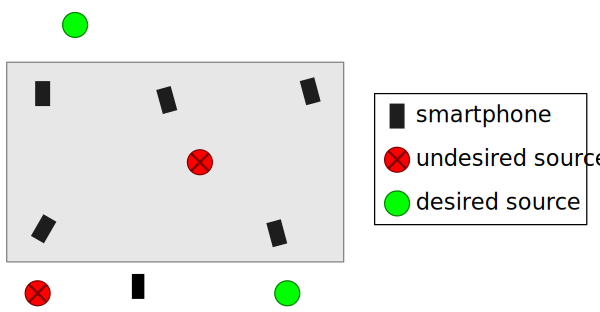
\includegraphics[width=0.8\textwidth]{figures/introduction/goal_example}
\caption[Typical usage scenario for the beamforming system.]{Typical usage scenario for the beamforming system. Several smartphones are positioned on a table to capture desired audio sources, while rejecting sources of noise.}
\label{fig:goal_example}
\end{figure}


\subsection{Scope}
This work describes a complete system for sensor data acquisition, taking the form of an Android smartphone application and a \matlab and Java processing server. An overview of the components of this system is shown in Fig.~\ref{fig:local_overview}. The choices for these platforms will be outlined in sections \ref{sec:android} and \ref{sec:matlab} respectively.

This work will also look at the state of the art of both orientation estimation and localization and make some recommendations for future work. It was chosen not to incorporate this functionality in the application, but instead assume the smartphone orientations and positions are known.

The following section details the definitions and mathematical symbols used in the rest of this work. A set of requirements for this subsystem follows in section \ref{sec:requirements}.

\section{Definitions and symbols}
Throughout the rest of this document, some shorthand form of long product names will be used. Below, these are enumerated and explained. The shorthand forms are also introduced.
\begin{description}[labelwidth=4cm]
\item[Android\texttrademark~platform]	Smartphone operating system -- abbreviated as Android. 
\item[Google Nexus 5\texttrademark]	Smartphones used in this work -- abbreviated as Nexus 5.
\item[MATLAB Student R2014b]		Numerical computing environment -- abbreviated as \matlab.
\item[Java\textregistered]		Programming language maintained by Oracle Corporation -- abbreviated as Java.
\end{description}

\subsection{Mathematical symbols}
The following mathematical symbols are used throughout this document:
\begin{description}[labelwidth=1.5cm]
\item[$\vec{a}, \vec{A}$]	time-domain and discrete-frequency-domain vector, respectively
\item[$\mathcal{F}$]	the discrete Fourier transform (DFT) operator, i.e. $\mathcal{F}\{\vec{f}~[t]\}=\vec{F}~[2\pi k/N]$
\item[$\fourier$]	the right-side element is the DFT of the left-side element, i.e. $\vec{f}~[t]~\fourier~\vec{F}~[2\pi k/N]$.
\item[$\vec{a} \star \vec{b}$]	the cross correlation between $\vec{a}$ and $\vec{b}$.
\item[$\vec{a} * \vec{b}$]		the convolution of $\vec{a}$ and $\vec{b}$.
\item[$a\cdot b$]	the product of $a$ and $b$.
\item[$\vec{a} \odot \vec{b}$]	the element-wise multiplication of $\vec{a}$ and $\vec{b}$.
\item[$\overline{a}$]	the complex conjugate of $a$.
\item[$0.\overline{1}$]	a recurring decimal, i.e. $0.111\dots$
\item[$\hat{a}$]	an estimate for $a$.
\end{description}

\begin{figure}[bht]
	\centering
	\begin{subfigure}{0.8\textwidth}
	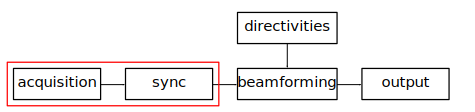
\includegraphics[width=\textwidth]{figures/introduction/global_overview}
		\caption[Global overview of the beamforming system structure.]{A global overview of the beamforming system structure. This work describes the stages highlighted in red.}
		\label{fig:global_overview}
	\end{subfigure}
	
	\begin{subfigure}{0.8\textwidth}
		\includegraphics[width=\textwidth]{figures/introduction/local_overview}
		\caption[General outline of system structure in this work.]{A closer look at the general outline of the system described in this work.}
		\label{fig:local_overview}
	\end{subfigure}
	\caption{Global and local overview of the beamforming system.}
\end{figure}


\section{Requirements}
\label{sec:requirements}
A set of requirements has been established before the subsystem was implemented, in order to judge if the finished subsystem complies with expectations. In the rest of this chapter, \emph{system} will refer to the complete, integrated system of smartphones and processing computer. 

\subsection{Requirements concerning the intended use}
	\paragraph*{}
\textbf{Requirements concerning the Android application.}
\begin{enumerate}
\item The Android application must have an easy-to-use graphical interface.
\item The Android application must connect using TCP/IP to a running server that will accept the recorded audio data.
\item The Android application must stream the data acquired from its microphone after receiving the corresponding signal from the central computer.
\item The Android application must stop streaming the recorded sound after receiving a stop signal.
\item The Android application must adhere strictly to the defined communication protocol with the central computer.
\end{enumerate}

\textbf{Requirements concerning the \matlab application.}
\begin{enumerate}
\item The \matlab program must accept incoming network connections from smartphones so data can be transmitted between them.
\item The \matlab program must be capable of handling 8 simultaneous phone connections.
\item The \matlab program must adhere strictly to the defined communication protocol with the phones.
\item The \matlab program must provide the beamforming algorithms with discrete, synchronized `blocks' with predefined size of sampled audio data from all phones.
\item The \matlab program must also provide a unique phone identifier to the beamforming algorithms along with the aforementioned audio data.
\end{enumerate}

\subsection{Requirements concerning the system}
\begin{enumerate}
\item The system must be usable in a typical office environment (e.g. a meeting room).
\item The Android application must run on Nexus 5 smartphones.
\item The computer program must run on computers running \matlab version R2014b with networking capability.
\end{enumerate}

\subsection{Requirements regarding the production}
\begin{enumerate}
\item The Android application will be developed using version 24.2 of the Android SDK\footnote{Software Development Kit}.
\item The \matlab code will be developed using \matlab version R2014b.
\item Java applications will be developed using version 1.7.0 of the JDK\footnote{Java Development Kit.}.
\end{enumerate}


\end{document}
